% Basic explanation of NN
In this thesis, we deal only with feed-forward neural networks, which are essentially directed acyclic graphs (DAG) for computation. In other words, information only moves through the network in one direction. An example neural network is shown in Figure \ref{fig:nn}.

\begin{figure}[!ht]
\centering
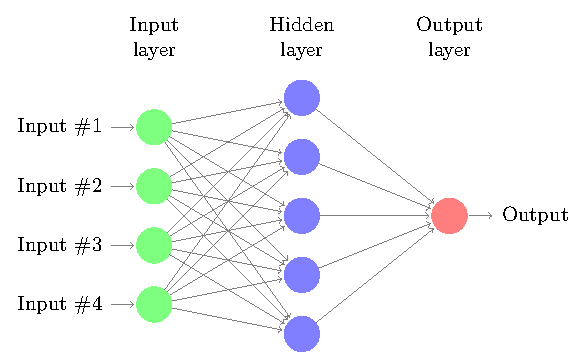
\includegraphics[width=.8\textwidth]{neural-network-texexample-net}
\caption[Example neural network]{An example neural network. There are 4 input variables, 1 hidden layer with 5 neurons, and 1 output variable.}
\label{fig:nn}
\end{figure}

The connections in a nerual network can be represented by linear combinations of the input variables with learned weights $\vec{w}$. \cite{bishop} Unlike standard linear models however, neural networks apply a nonlinear activation $f(\centerdot)$ at the output of each neuron. The circle nodes in a neural network diagram can be thought of as the sum of the linear combinations of the connection edges and the application of the bias and activation function. Therefore, a hidden neuron $z_{j}$ in a network with $N$ input variable nodes, $M$ hidden nodes, and $K$ output nodes takes on the value

\begin{equation}
z_j = f(a_j)
\end{equation}

where the activiation $a_j$ is given by

\begin{equation}
a_j = \sum_{i=1}^{N} w_{ji}^{(1)}x_i + w_{j0}^{(1)}
\end{equation}

The connection values $w_{ji}$ are referred to as weights, and the scalars $w_{j0}$ are referred to as biases. Note that the superscripted numbers refer to the Then, the output $y_{k}$ is given by

\begin{equation}
y_k = g(a_k)
\end{equation}

where the output activation $a{k}$ is given by

\begin{equation}
a_k = \sum_{j=1}^{M} w_{kj}^{(2)} z_j + w_{k0}^{(2)}
\end{equation}

We are free to choose activation functions, which we will discuss later. However, note that at the output, the function $g(\centerdot)$ is often an identity for regression problems and a sigmoid $\sigma(\centerdot)$ for classification problems.

Often, the weights and biases are grouped into a weight vector $\vec{w}$. In other words, similar to the linear models described earlier, a neural network is a nonlinear function of input variables $\{x_i\}$ to output variables $\{y_k\}$ where the parameters of the function are learned via training techniques.

\subsubsection{Dense Layer}

Described in the previous section, we refer to a dense layer as a fully connected neural network, in which no interconnections between neurons are missing at each layer. Dense layers can be prone to overfitting. However, as we mention later, overfitting is not an immediate concern for the purposes of this thesis.

\subsubsection{Autoencoder}

An autoencoder is

\subsubsection{Convolutional Layer}



\subsubsection{Nonlinearity Choice}



\subsubsection{Minibatches}



\subsubsection{Batch Normalization}



\subsubsection{Weight Updates}


% \subsubsection{Neural networks as computational graphs}

% A neural network generally is a computational graph $G = (V, E)$ where the
% vertices $V$ correspond to nodes of computation, and the edges $E$ correspond
% to data flow paths connecting the computational nodes. We limit our discussion
% to feed-forward or directed acyclic graphs, in other words graphs where given
% a starting vertex $v$ we are unable to follow the directed edges away from it
% and return to $v$. With this limitation in place we are able to focus on
% stateless graphs, which treat input data examples independently of one another.

% With the additional limitation that all computational nodes in the graph
% perform differentiable operations, and that some nodes are parametric, we are
% able to use automatic differentiation and a gradient descent like optimization
% algorithm to optimize the parameters of the graph against a differentiable
% loss function \cite{DBLP:journals/corr/BaydinPR15}. Automatic differentiation
% is an alternative to numeric and symbolic differentiation, that is efficient,
% accurate to machine precision, and scalable to arbitrary graphs consisting of
% elementary operations. The core tenet of automatic differentiation is that
% since graph vertices are differentiable we can perform the chain rule at each
% node to build up gradients of the full graph. Several machine learning
% frameworks, such as Theano and TensorFlow implement automatic differentiation,
% allowing us to specify the functional form of the graph and getting gradients
% at minimal cost \cite{bergstra-proc-scipy-2010,DBLP:journals/corr/AbadiABBCCCDDDG16}.

% \subsubsection{Fully connected neural networks}
% \label{sec:nn}

% While we have introduced the idea that neural networks can be made up of
% arbitrary computational nodes, there are several common types of nodes that
% are used to build up a toolkit of functional forms at our disposal. First, let
% us a consider a simple inner product with signature:
% \begin{equation}
% \langle \cdot, \cdot \rangle \colon \mathbb{R}^n \times \mathbb{R}^n \to \mathbb{R}
% \end{equation}
% And functional form:
% \begin{equation}
% \langle \mathbf{w}, \mathbf{x} \rangle = \sum\limits_{i = 1}^n w_ix_i
% \end{equation}

% We can interpret this inner product as a single node in our graph, with
% parameters $\mathbf{w}$ and input vector $\mathbf{x}$. While this functional
% form is nice, in that it's linear, and easy to define, it's limited by the
% fact that it brings the rich space $\mathbb{R}^n \times \mathbb{R}^n$ down to
% $\mathbb{R}$ which has limited representational power for problems of interest
% in machine learning. Instead we'll follow a common design pattern, and create
% an array of inner product nodes at a constant number of hops from the source node
% in the graph, or as we'll refer to from here on, at a constant depth. In this case the signature would be:
% \begin{equation}
% g \colon \mathbb{R}^{n \times m} \times \mathbb{R}^n \to \mathbb{R}^m
% \end{equation}
% And functional form:
% \begin{equation}
% g\left(W, \mathbf{x}\right)_j = \sum\limits_{i=1}^n w_{ij}x_i
% \end{equation}
% which we recognize as ordinary matrix multiplication $W\mathbf{x}$, where $W
% \in \mathbb{R}^{n \times m}$. We call this collection of nodes at a common
% depth a layer. This type of matrix multiplication layer is generally referred to
% as a linear, dense, or fully connected layer.

% Layers can be connected together with the goal of creating a more powerful model.
% If we feed one dense layer into another directly we have have a functional form:
% \begin{equation}
% \mathbf{y} = W_n \cdots W_3W_2W_1\mathbf{x}
% \end{equation}

% where the $W_i$'s are all compatible. However this approach is actually
% equivalent to a single matrix multiply $W\mathbf{x}$ where $W$ is the matrix
% product of the $W_i$'s, so we did not actually achieve our goal of higher
% representational power. Our model is still merely linear.

% To address this issue the we introduce the addition of a non-linear
% transformation $f(\cdot)$ (known as an activation function) at the output of
% the matrix multiply. So instead our functional form would be:
% \begin{equation}
% \mathbf{y} = f(W_n \cdots f(W_3f(W_2f(W_1\mathbf{x})))\cdots)
% \end{equation}
% As long as $f(\cdot)$ is differentiable we are able to train our now highly
% non-linear model with our methods of automatic differentiation and gradient
% based optimization.

% Finally we introduce a bias $\mathbf{b}$ so that each node in a layer is not
% constrained to intercept zero. Therefore our full functional form for a single fully
% connected layer with a non-linearity is:
% \begin{equation}
% \mathbf{y} = f\left(W\mathbf{x} + \mathbf{b}\right)
% \label{dense}
% \end{equation}
% with $W \in \mathbb{R}^{n\times m}$ and $\mathbf{b} \in \mathbb{R}^m$.

% A traditional activation function is the sigmoid function:
% \begin{equation}
% S(t) = \frac{1}{1 + e^{-t}}
% \end{equation}

% which maps $t \in \mathbb{R}$ (i.e the interval $[-\infty, \infty]$) to $S(t)$
% on the interval $[0,1]$. This can allow the interpretation of $S(t)$ as a
% probability. Using this activation function Cybenko proved the universal
% approximation theorem \cite{cybenko1989approximation} which shows that neural
% networks of the form in Figure \ref{densenn} can approximate any function with
% appropriate domain and codomains given a large of enough number nodes in the
% middle layer, generally referred to as a hidden layer.

% \begin{figure}
% \begin{center}
% \begin{tikzpicture}[
plain/.style={
  draw=none,
  fill=none,
  },
net/.style={
  matrix of nodes,
  nodes={
    draw,
    circle,
    inner sep=5pt
    },
  nodes in empty cells,
  column sep=-0.5cm,
  row sep=-5pt
  },
>=latex
]
\matrix[net] (mat)
{
|[plain]| \parbox{1.3cm}{\centering Input\\layer} & |[plain]| \parbox{1.3cm}{\centering Hidden\\layer} & |[plain]| \parbox{1.3cm}{\centering Output\\layer} \\
& |[plain]| \\
|[plain]| & \\
& |[plain]| \\
|[plain]| & |[plain]| \\
& & \\
|[plain]| & |[plain]| \\
& |[plain]| \\
|[plain]| & \\
& |[plain]| \\
};
\foreach \ai [count=\mi ]in {2,4,...,10}
  \draw[<-] (mat-\ai-1) -- node[above] {$x_\mi$} +(-2cm,0);
\foreach \ai in {2,4,...,10}
{\foreach \aii in {3,6,9}
  \draw[->] (mat-\ai-1) -- (mat-\aii-2);
}
\foreach \ai in {3,6,9}
  \draw[->] (mat-\ai-2) -- (mat-6-3);
\draw[->] (mat-6-3) -- node[above] {Ouput} +(2cm,0);
\end{tikzpicture}
% \end{center}
% \caption[Feed-forward fully-connected network]{A single hidden layer feed-forward neural network. Each directed
% connection has a scaling factor $w_{ij}$ associated with it; these entries make
% up the $W$ matrix. Each circle, now referred to as a neuron, performs the
% sum and activation functions corresponding to the matrix multiply, and
% mapping by $f(\cdot)$ in Equation \ref{dense}. Layers in the middle of the
% network are referred to as hidden layers because they are not directly observable
% --- instead these are latent variables.}
% \label{densenn}
% \end{figure}

% Figure \ref{densenn} shows a feed-forward network with one hidden-layer. The
% outputs of the hidden layer are referred to as latent variables and are a new type of
% representation for the input data $\mathbf{x}$. With each hidden-layer added to
% the network increasingly complex data representations may be available, but the
% networks will also tend to over-fit their training data as the number of
% parameters increase. In order to combat over-fitting, and increase the
% generalization performance of the network new types of architectures have been
% proposed.


% \subsubsection{Convolutional neural networks}
% % The first convolutional neural network was proposed by Fukushima in 1980 \cite{conv}.
% % The idea of the network is that instead of creating a weight matrix $W$ with
% % parameters that correspond to every entry in $\mathbf{x}$, that there would be a
% % kernel of some small size that would be swept across across $\mathbf{x}$. This
% % process is essentially a convolution. Mathematically this process is:
% % \begin{equation}
% % \mathbf{y} = f(\mathbf{x} \star \mathbf{w})
% % \end{equation}
% % Where $\star$ represents a discrete convolution, $\mathbf{w}$ is a
% % one-dimensional kernel and $f(\cdot)$ is an activation function. This method can
% % be extended to work for two and three-dimensional data representations, for
% % example:
% % \begin{equation}
% % Y = f(X \star W)
% % \end{equation}
% % where $Y,X$ and $W$ are all matrices.
% \subsubsection{Convolutions with holes}
% \subsubsection{Tranposed convolutions}
% \subsubsection{Additional techniques}
% \paragraph{Dropout}
% Various teams have demonstrated that in deep networks neurons can learn
% complex co-adaptation schemes; that is deep neurons respond to ``mistakes'' in
% shallower neurons. In order to prevent co-adaptation, so that each neuron
% learns a meaningful representation, the dropout scheme has been proposed
% \cite{JMLR:v15:srivastava14a,DBLP:journals/corr/abs-1207-0580,dahl2013improving}.
% Dropout is a masking process. In order to apply dropout to a layer during
% training, a binary mask is applied across neurons. The mask is determined by
% sampling a Bernoulli distribution with a parameter $p$ corresponding to the
% probability that a neuron will be masked. When a neuron is masked its output
% is considered fixed at zero. When the network is used for evaluation no masks
% are applied and all neurons are connected.
% \paragraph{Batch normalization}
% \paragraph{Rectified linear units}
% Various activations have been proposed on the basis of similarity to the
% potential activations in actual biological neurons in human eyes. Recently the
% rectified linear unit (ReLU) has demonstrated significant performance
% increases for network generalization and increased training speed
% \cite{glorot2011deep,dahl2013improving}. The ReLU activation is defined as
% $\text{max}(0,x)$. In other words a ReLU activation forwards along any
% positive inputs and sets and negative inputs to zero.
% \paragraph{Exponential linear units}
% \paragraph{Residual networks}
% \paragraph{Minibatch training}
% Traditionally there were two different approaches to optimizing neural
% network parameters, the online approach and the batch approach. In the online
% approach, the parameters of the network are updated after each exposure to a
% training example and gradient calculation. In the batch approach, the network
% is exposed to all of the training examples, the gradients are accumulated and
% then the network's parameters are updated. This was long believed to be the
% better approach, as the accumulated and averaged gradient was more likely to
% be an estimate of the ``true'' gradient of the network towards an optimized
% solution. It was later shown  that, while the batch mode may give a better
% estimate of the gradient, due to the noise and its stochastic nature, the
% online approach actually leads to a faster convergence time, in terms of
% number of examples \cite{Wilson:2003:GIB:965268.965272}. This is because in
% the stochastic approach the optimizer is less likely to get stuck in local
% minima. An alternative approach that recently has become popular is the mini-
% batch approach. In this approach some number of examples, say $N$, are exposed
% to the network, the gradients are accumulated, and the parameters are updated.
% In this case $N$ is much less than the total number of training examples
% available. This approach, with serial computational resources really only
% represents a decrease in training speed, because it is fairly similar to the
% batch approach. The reason this approach has become popular lately is that
% with the parallel resources afforded by modern high performance graphics
% processing units (GPUs) the increase in example-wise training time becomes a
% decrease in wall-time to train.

% \paragraph{Intelligent parameter initialization}
% Kaiming et al. have demonstrated an improved parameter initialization
% technique specifically designed for neurons with ReLU activations
% \cite{DBLP:journals/corr/HeZR015}. This approach derives a method that enables
% extremely deep models comprised of ReLU neurons to converge rather than stall,
% as they would with other initialization schemes. The initial parameters for
% the convolutional layers are drawn from a zero mean normal distribution with a
% standard deviation of  $\sqrt{2/n_l}$. Where $n_l = k^2c$. This corresponds to
% the number of connections in the response for $k\times k$ kernels processing
% $c$ input channels.

% \paragraph{ADAM optimizer}
% \paragraph{Style loss}
